\documentclass[onecolumn, draftclsnofoot,10pt, compsoc]{IEEEtran}
\usepackage{graphicx}
\usepackage{url}
\usepackage{setspace}

\usepackage{listings}
\usepackage{xcolor}

\usepackage[T1]{fontenc}
\usepackage[scaled]{beramono}

\usepackage{color}
\definecolor{bluekeywords}{rgb}{0.13,0.13,1}
\definecolor{greencomments}{rgb}{0,0.5,0}
\definecolor{redstrings}{rgb}{0.9,0,0}

\lstset{language=[Sharp]C,
showspaces=false,
showtabs=false,
breaklines=true,
showstringspaces=false,
breakatwhitespace=true,
escapeinside={(*@}{@*)},
commentstyle=\color{greencomments},
keywordstyle=\color{bluekeywords}\bfseries,
stringstyle=\color{redstrings},
basicstyle=\ttfamily
}

\usepackage{geometry}
\geometry{textheight=9.5in, textwidth=7in}

% 1. Fill in these details
\def \CapstoneTeamName{			Velocity-Raptors}
\def \CapstoneTeamNumber{		37}
\def \GroupMemberOne{			Alex Bailey}
\def \GroupMemberTwo{			Dylan Washburne}
\def \GroupMemberThree{			Benjamin Wick}
\def \CapstoneProjectName{		Object Velocity Tracking}
\def \CapstoneSponsorCompany{}
\def \CapstoneSponsorPerson{		Alex Neighbors}

% 2. Uncomment the appropriate line below so that the document type works
\def \DocType{		%Problem Statement
				%Requirements Document
				%Technology Review
				%Design Document
				Progress Report
				}
			
\newcommand{\NameSigPair}[1]{\par
\makebox[2.75in][r]{#1} \hfil 	\makebox[3.25in]{\makebox[2.25in]{\hrulefill} \hfill		\makebox[.75in]{\hrulefill}}
\par\vspace{-12pt} \textit{\tiny\noindent
\makebox[2.75in]{} \hfil		\makebox[3.25in]{\makebox[2.25in][r]{Signature} \hfill	\makebox[.75in][r]{Date}}}}
% 3. If the document is not to be signed, uncomment the RENEWcommand below
\renewcommand{\NameSigPair}[1]{#1}

%%%%%%%%%%%%%%%%%%%%%%%%%%%%%%%%%%%%%%%
\begin{document}
\begin{titlepage}
    \pagenumbering{gobble}
    \begin{singlespace}
    	
\includegraphics[height=4cm]{coe_v_spot1}
        \hfill 
        % 4. If you have a logo, use this includegraphics command to put it on the coversheet.
        %\includegraphics[height=4cm]{CompanyLogo}   
        \par\vspace{.2in}
        \centering
        \scshape{
            \huge CS Capstone \DocType \par
            {\large\today}\par
            \vspace{.5in}
            \textbf{\Huge\CapstoneProjectName}\par
            \vfill
            {\large Prepared for}\par
            \Huge \CapstoneSponsorCompany\par
            \vspace{5pt}
            {\Large\NameSigPair{\CapstoneSponsorPerson}\par}
            {\large Prepared by }\par
            Group\CapstoneTeamNumber\par
            % 5. comment out the line below this one if you do not wish to name your team
            %\CapstoneTeamName\par 
            \vspace{5pt}
            {\Large
                \NameSigPair{\GroupMemberOne}\par
                \NameSigPair{\GroupMemberTwo}\par
                \NameSigPair{\GroupMemberThree}\par
            }
            \vspace{20pt}
        }
        \begin{abstract}
        % 6. Fill in your abstract    
        	This document is intended to give an update for the progress of our project.
            It includes goals, project status, pieces of interesting code to share, and screen shots.
            
        \end{abstract}     
    \end{singlespace}
\end{titlepage}
\newpage
\pagenumbering{arabic}
\tableofcontents
% 7. uncomment this (if applicable). Consider adding a page break.
%\listoffigures
%\listoftables
\clearpage

% 8. now you write!
\section{Project Purpose and Goals}
The overall purpose of our project is to use a stationary camera to detect moving objects and then determine the velocity at which the objects are moving which will be displayed to the user.
This project is intended to be a proof of theory where future larger scaled systems can then be implemented based off our smaller scaled project.
In theory, the objects can be anything the user wishes to track which can include, but not limited to, vehicles, people, sports objects, animals and any other moving objects the user wishes to track.

There can be many different applications over many different fields for this kind of system.
An example is using the system to monitor the average speed at which cars are traveling on the freeway.
This system can be implemented using different cameras and hardware to meet the needs of the user.

This system offers an alternative to current speed tracking methods like radar guns.
The benefit of our system is that it is capable of tracking the speed of objects unmanned.
This means that someone simply needs to set it up and the data for the objects speed can be viewed later on.

In the case of our project, we used a Microsoft Kinect to track the motion of a red ball and calculate the speed at which it is moving.

The goal of our project is to create a working prototype with a friendly user interface in the form of a Microsoft Windows application which will display the video feed and speed.
Accuracy and reliability is another goal important goal we intend to accomplish.

\section{Current Status of Project}
We have made a lot of progress since the beginning of our project. Currently we have a working prototype of our system that can track a red ball. Once it tracks the red ball it is able to draw a red circle and calculate the position of the ball which is the x and y coordinate. We also have a depth map generated by the Kinect. With all of this information we are able to calculate the speed of the red ball. This is all done by using a Microsoft Kinect camera and EmguCV for computer vision. We also have a feature that outputs the x coordinate, y coordinate, depth data, and the speed of the object into a text document. We have a recording feature that saves every frame but we decided not to include this in our final product because it caused performance issues.


\section{Work Remaining}
Technically speaking, we do not have any work remaining, as we created a minimum viable product before the code freeze, and will continue to stand by our program.  That said, there are features we would still like to include at a smaller scale.

First, we would like to polish up the user interface.  Our current UI isn't strictly speaking bad, but it does suffer from being generic and, frankly, ugly.  We could spend time to improve the visuals and overall structure of the UI, but we have not spent time on that so far because we were more concerned with function over form.

We would also like to resolve an issue where the program works at much lower efficiency on some architectures.  We have not isolated this issue yet, so we do not yet know what is needed to resolve this issue.  We have only thus far spent a small amount of time on the issue, because we were able to circumvent it on certain computers.  If we were to continue forward with the program, this would be a high-priority issue to fix.

We would also like to implement a system to save and playback our object tracking.  This was a system we had planned for since the beginning, but we cut it near the end due to issues introduced by attempting to save, and the fact it wasn't strictly speaking a piece of the minimum viable product.  We would still like to implement this feature, but it did not make the cut for the expo.

\section{Problems}
During our work this term, one of our big problems was that we realized that the things that we planned to do in our design document would be very difficult to finish in the time that we had remaining.
One thing was that we intended to track people as they passed by, but we found this to be harder than originally anticipated.
Instead, we received permission to use a red ball for our tracking.
Another problem we realized is that tracking multiple objects would be difficult.
We weren't able to figure out a way to determine which object in one frame would correspond to which object in the next frame, when multiple objects were in frame.
We also realized that 90\% accuracy would be difficult.
Originally, when we were thinking about tracking cars, since they were traveling relatively fast, 90\% would be more attainable.
However, since the ball we are tracking is move, at most, a couple of miles an hour, this would mean that our speed would have to be within about .3 mph of the true value, which would be very difficult.

A more technical problem that came up in our project was the recording feature.
It seemed that this feature may have been more that our computers were capable of handling, as this would cause the live feed to not be displayed.
Considering that act of tracking the ball could already cause the frame rate to lower, this seemed to make sense.
Another technical problem that we ran into is that for an unknown reason, when we installed our code onto a certain computer, the live video feed would not show unless the tracking algorithm was removed.
We were able to get our code working on other computers, and due to our limited time we were unable to narrow down the problem.


\section{Pieces of Code}
This function includes the bulk of our program's logic. It includes the EmguCV calls to track the object as well as calculating the speed. Because those are the main parts of these functions, other pieces of code have been removed to make it more condensed within the function.
The comments within the code will give an explanation of what is going on.
\begin{lstlisting}
        void ProcessFrame()
        {
            // Convert the Bgr image to an HSV (hue, saturation values) image. This is important because we need to be able to find the range of values in order to track the object by color.
            CvInvoke.CvtColor(originalImage, hsvImage, ColorConversion.Bgr2Hsv);

            // This creates a range of hue values for red and then adds both to the processedImage. This is where we are tracking the red in frames. The processedImage frame is creating a seperate threshold image of just the red pixels in which we are tracking.
            CvInvoke.InRange(hsvImage, new ScalarArray(new MCvScalar(0, 155, 155)), new ScalarArray(new MCvScalar(20, 255, 255)), lower_red_hue_range);
            CvInvoke.InRange(hsvImage, new ScalarArray(new MCvScalar(160, 155, 155)), new ScalarArray(new MCvScalar(179, 255, 255)), upper_red_hue_range);
            CvInvoke.Add(lower_red_hue_range, upper_red_hue_range, processedImage);

            // This is where we draw the circles around the object in the frame in the Original image.
            foreach (CircleF circle in circles)
            {
                CvInvoke.Circle(originalImage, new Point((int)circle.Center.X, (int)circle.Center.Y), (int)circle.Radius, new MCvScalar(0, 0, 255), 2);
                CvInvoke.Circle(originalImage, new Point((int)circle.Center.X, (int)circle.Center.Y), 3, new MCvScalar(0, 255, 0), -1);
            }

            // Each frame, this function as a whole gets called.  As a result, it is able to affect the globally declared 'tick' variable, which is what we use to reduce the frequency of speed calculations to only a specific number of calculations per second, at what we call the tick rate
            tick--;
            if (circles != null && circles.Length != 0)
            {
                x_pos = (int)circles[0].Center.X;
                y_pos = (int)circles[0].Center.Y;
                z_pos = (ushort)depth_data[(depth_data_width * (int)circles[0].Center.Y) + ((int)circles[0].Center.X)] >> 3;

                double x_disp, y_disp, z_disp;

                // If an object is getting tracked in-frame and we have hit a point that is at minimum one tick later than the previous tick, we can run a velocity calculation.
                if (tick <= 0)
                {
                    tick = tick_rate;

                    // The displacement in x and y is "scaled" due to its position in z space, so we multiply the variables at this point.
                    x_disp = (x_pos - x_prev) * z_pos;
                    y_disp = (y_pos - y_prev) * z_pos;
                    z_disp = Math.Pow(z_pos - z_prev, 2);
                    
                    // The speed calculation is essentially finding the Pythagorean theorem of x, y, and z displacement, then divided from millimeters to feet.
                    double speed = ((Math.Sqrt(Math.Pow(x_disp, 2) + Math.Pow(y_disp, 2) + Math.Pow(z_disp, 2))) / 304.8 / 304.8 * (10));

                    this.speed_val_label.Text = speed.ToString();

                    x_prev = x_pos;
                    y_prev = y_pos;
                    z_prev = z_pos;
                }
            }

            imageBox1.Image = originalImage;
        }
\end{lstlisting}

\section{Hardware}
We chose to use the Microsoft Xbox 360 Kinect. The Kinect has an RGB camera as well as two 3D depth sensors. These depth sensors should help us create a depth map that can be used to determine the distance of a person on the screen, which will be vital in determining speed.
\newline
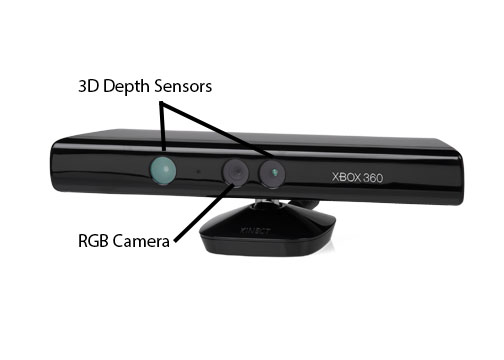
\includegraphics[height=5.5cm]{kinect1}
\newline
The Kinect was made for the Xbox 360 which meant we had to buy an adapter that will allow us to plug it into a female USB port. Below is an image of the adapter that will be used to do so.
\newline
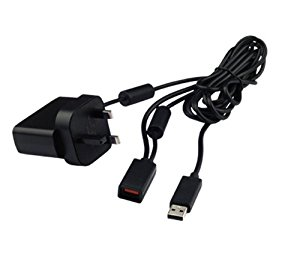
\includegraphics[height=5.5cm]{adapter}
\newline
Both these hardware components aren't necessary for every system to be implemented.
Theoretically, other cameras may be used depending on the object being tracked.
We chose to use the Kinect because of price, convenience, and the ability to detect people.
The combination of these two hardware pieces will allow us to create a live video for our program to detect objects which will help us obtain our goal.

\section{User Interface}
The screen shot below is an example of our user interface. You can see the red circle being tracked as well as the data being displayed.
\newline
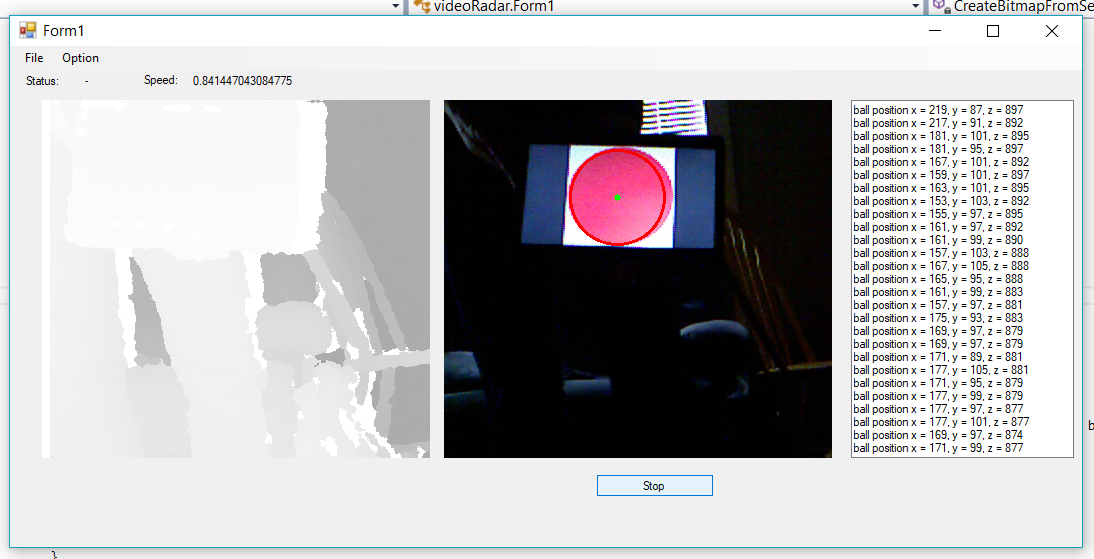
\includegraphics[height=9cm]{ui}
\newline
Below is also an example of what the output of the data file looks like. The data is comma separated in the following order; x-coordinate, y-coordinate, depth data, and finally speed.
\newline
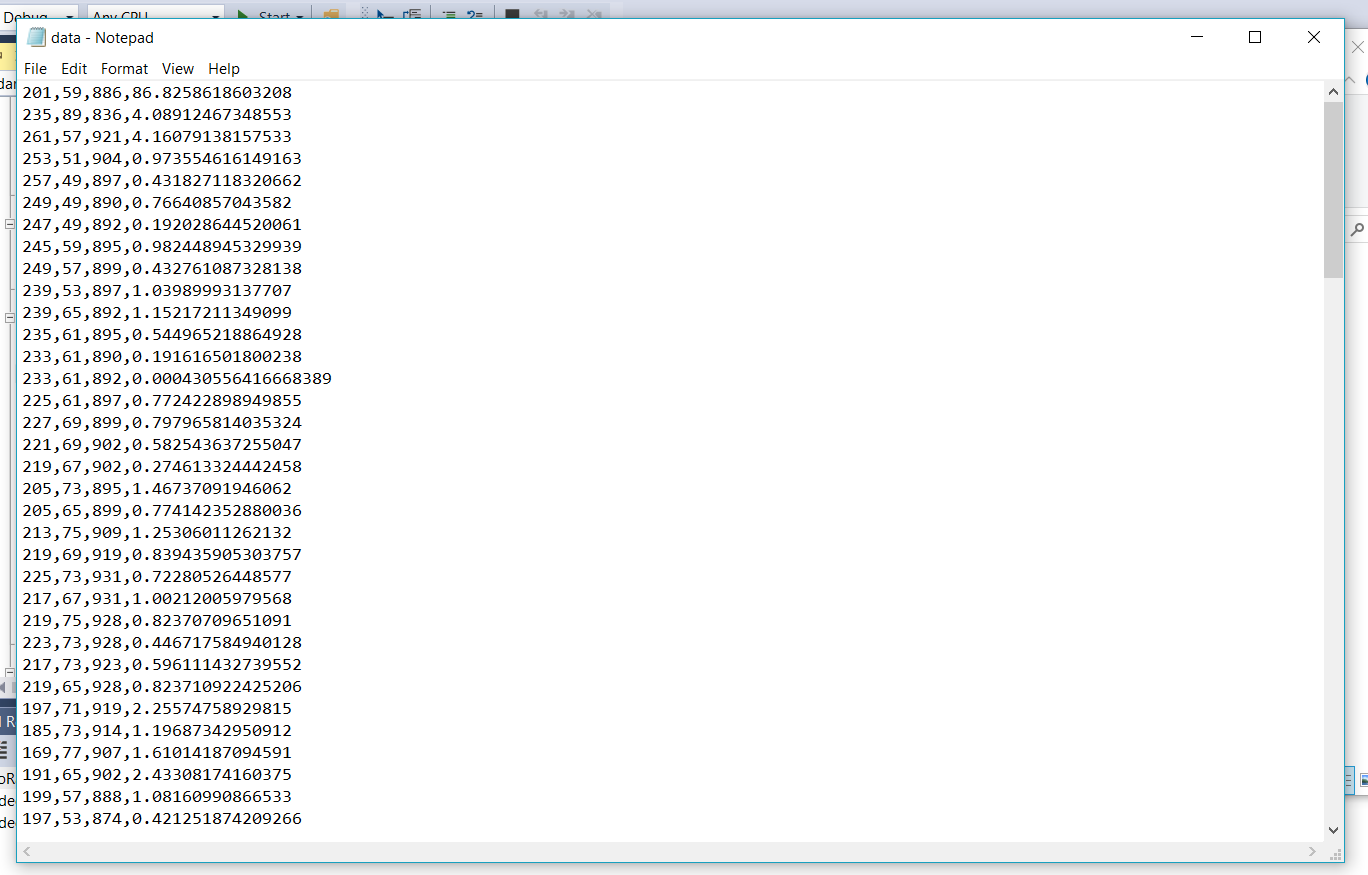
\includegraphics[height=9cm]{data}
\newline
The image below shows an example of what our recording feature looks like. It records each frame and saves them into a folder.
\newline
\newline
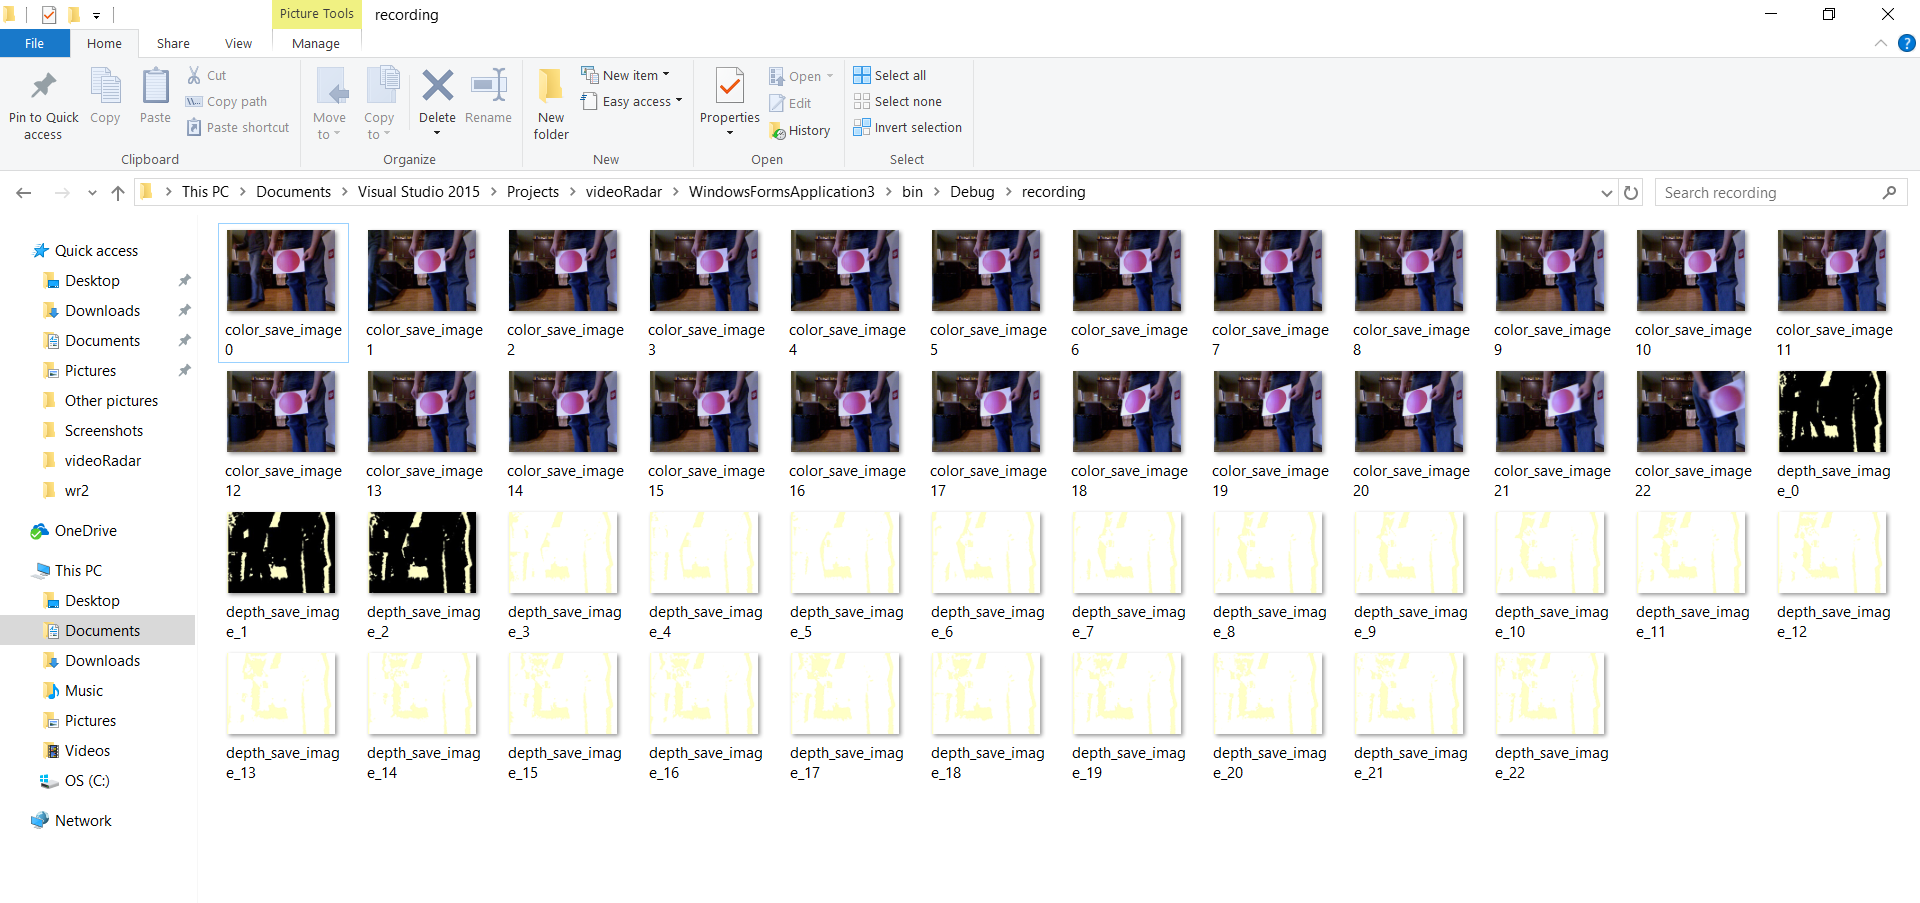
\includegraphics[height=9cm]{saving}


\end{document}